\documentclass[11pt]{article}
\pdfoutput=1

%all the ams math symbols
\usepackage{amsmath,amssymb,amsbsy,amstext, amsthm, amsfonts,amssymb,simplewick}
%needed for linking to websites
\usepackage{hyperref}
%Needed for figures (at least the way I implement them below)
\usepackage{graphicx}

%Some basic layout commands (sets margins at line spacing)
\setlength{\textwidth}{460pt}
\setlength{\topmargin}{-1.2cm} \setlength{\textheight}{640pt} \setlength{\oddsidemargin}{10pt} \linespread{1.1}

% Here we set how our equations are going to be numbered - here we number by section (1.1-1.N, then 2.1, ... etc).
\numberwithin{equation}{section}
%If we remove this command the equations would just be 1 - N for the whole document

%We could make similar commands for figures and tables.  Since we typically have few figures and tables, we will just label them 1 to N.

\def\beq{\begin{equation}}
\def\eeq{\end{equation}}

\def\bea{\begin{eqnarray}}
\def\eea{\end{eqnarray}}



\def\cO{{\cal O}}

\def\Mp{M_{\rm pl}}

% Here is some user defined command
\newcommand{\vev}[1]{\langle #1 \rangle}
%To use it, we would write \vev{something} and it interprets it as \langle something \rangle


%%%%%% This is the start of the document %%%%%%%%%%%%%
\begin{document}


\begin{titlepage}


\begin{center}

{\fontsize{20}{28}\selectfont  \sffamily \bfseries A Template for} {\fontsize{20}{28}\selectfont   \LaTeX}

\end{center}

\vspace{0.2cm}

\begin{center}
{\fontsize{14}{18}\selectfont  Daniel Green}
\end{center}
%This takes the form \fontsize{size}{baselineskip} - Baselineskip is mostly irrelevant unless you are writing multiple paragraphs.

\begin{center}
\textsl{ Canadian Institute for Theoretical Astrophysics, Toronto, ON M5S 3H8, Canada}
% italics (one of many types of italics)
\end{center}


\vspace{1.2cm}
\hrule \vspace{0.3cm}
\noindent {\sffamily \bfseries Abstract}
This is an abstract
\vskip 10pt
\hrule

\vspace{0.6cm}
\end{titlepage}


\tableofcontents

\newpage 


\section{Introduction}\label{sec:intro}

There are lots of ways to use latex.  I recommend download TexShop or something equivalent for you home computer / laptop.  This has a bunch of nice built in features for working with .tex files.

However, as long as you have .tex installed (as it is on the CITA cluster / lobster machines) you can write a latex document in any text editor (e.g. emacs) and then compile it to make the pdf file in the terminal using the command latex filename.tex.

\section{Basic Usage}\label{sec:basics}
This is a section.  To start a new section, subsection, subsubsection, you just put in the appropriate command where you want to start the new section.  Sometimes you may want to have a new section start on a new page so we would just write the command newpage like we did after the table of contents.
If you want to start a new paragraph, you need to put a full space in between the lines (just pressing enter/return is not enough).

This is a new paragraph.  Notice the automatic indent.

\noindent This is how you remove the automatic indent.

For the most part, writing text is latex is just like any text editor so for the most part you just write what you want, until you get to an equation, a figure, a new section, etc, where you will need a latex command.  However, there are a few issues that you should always remember.  First of all, quotation marks are a bit odd.  If you write "hi", it looks wrong in pdf even though it looks fine in the text editor.  What you need to write is ``hi" so that it gets treats the left and right quotes separately.

The second issue is that there are a few very special characters in latex that won't appear if you write them as usual.  Normally, you put the correct thing by adding a backslash : e.g. \{, \$, \}, \%.  Backslash is a very important one because it is used as the way to refer to a command.  A backlash on its own add a bit of space and two starts a new line: see\ this or this\\ won't work.  Instead I need \textbackslash.

We can use  pre-made commands like $\vev{t}$ or pre made variables like $\Mp$ or $\cO$.  These are inline equations.  If we want equations to be displayed we can use
\beq
\Delta S = \int_a^b \frac{d Q}{T}
\eeq
Or if we want to have a sequence of aligned equations, we use equation array
\bea
y&=&\sin(x+y) \\
&=& \sin(x) \cos(y)+ \cos(x) \sin(y)
\eea
Maybe we want to only have 1 numbered equation but we would like to have a reference to it in the text:\
\bea
y&=&\sin(x+y) \nonumber \\
&=& \sin(x) \cos(y)+ \cos(x) \sin(y) \label{giveitaname}
\eea
Most math functions as easy to look up.  Derivatives are often written
\beq
\frac{\mathrm d}{\mathrm d x} = \frac{\partial}{\partial_x} + \frac{\partial}{\partial y} \frac{\partial y}{\partial x} + \ldots
\eeq

Now we can refer to it in the text whenever we want, just by writing blah blah blah equation \ref{giveitaname} or (\ref{giveitaname}).  Notice that we also labelled the section title so that can say things like blah blah Section \ref{sec:intro}.  Never manually write equation 1.4 or section 1 because these things can change when you edit the document and you don't want to have to keep track of the changes.

Fractions can be written using $\frac{1}{2}$ and square roots are $\sqrt{a}$.

A common problem is double subscripts or subscripts.  Latex won't let do this twice, so you should be careful.  This is a bigger issue when you have both superscripts and subscripts as labels and then you want to take a power: $f_{\rm NL}^{\rm eq}{}^2$ or $f_{\rm NL}^{{\rm eq} \ 2}$.

To avoid having confusion over brackets, you have lots of options:
\beq
\Bigg[\Bigg(\bigg(\Big(\big((1+a)+a\big)+a\Big)+a\bigg)+a\Bigg)+\Big[\big[[1+a]+a\big]+a\Big]\Bigg]
\eeq
This gives you lots of control to highlight the brackets of interest.  In some cases, automatic sizing works just fine
\beq
(\frac{3}{4}) \neq \left( \frac{3}{4}\right)
\eeq
The option used on the right matches the size of the bracket to the object.

There are also lots of accents we can add to a given variable
\beq
\tilde a \vec a \dot a \ddot a a' \hat a
\eeq
The structure is that if you don't include brackets, it will apply the operation to the next character.  This is an issue, typically with exponents because it may not be obvious that you made a mistake because there is no error
\beq
a^{24} \neq a^24 \ .
\eeq
There are also lots of symbols available to use.  The greek alphabet is there $\alpha, \beta, \gamma, \ldots $ but also pretty much any math expression is defined
\beq
\sum_{i=1}^{n} \prod_{m=1}^{i} \varphi_{m} \gg 1
\eeq

Finally, this is how we cite papers : We can cite 2 papers \cite{Maldacena:2002vr,Ade:2013ydc}.


\section{Other useful tricks}

Let's start this section by making a list of things
\begin{itemize}
\item thing 1
\item thing 2
\end{itemize}
Or perhaps you want to enumerate the list
\begin{enumerate}
\item thing 1
\item thing 2
\end{enumerate}
For either of these, you can keep adding items to the list with the same format.

\subsection{Matrices}

Writing an equation with a matrix is slightly more work then what we have done so far. The most basic options is an array
\beq
\begin{array}{ccc}
a & b & c \\
d & e & f \\
g & h & i \end{array}
\eeq

\beq
\begin{array}{||c|c|c||}
a & b & c \\
d & e & f \\
g & h & i \end{array}
\eeq
\beq
\begin{array}{||c|c|c||}
a & b & c \\
\hline
d & e & f \\
g & h & i \end{array}
\eeq
We can also use automatic sizing to make this look like a matrix
\beq
\left(\begin{array}{ccc}
a & b & c \\
d & e & f \\
g & h & i \end{array}\right) = {\cal M}
\eeq

There are also direct matrix options 
\beq
\begin{pmatrix}
a & b & c \\
d & e & f \\
g & h & i \end{pmatrix} ={\cal M}
\eeq
The spacing here is a bit tighter than the above (may be preferable for an equation).

\subsubsection{This is a subsubsection}

\subsection{Figure}

The most annoying feature of latex is that it is very hard to put a figure exactly where you want it. The syntax is that you write begin\{figure\}[placement command].  There are a few placement commands: h (roughly where you put it in the tex file), t (top of page), b (bottom), ! (overrides LaTeX function for determining ``good positions").

\begin{figure}[h!]
\begin{center}
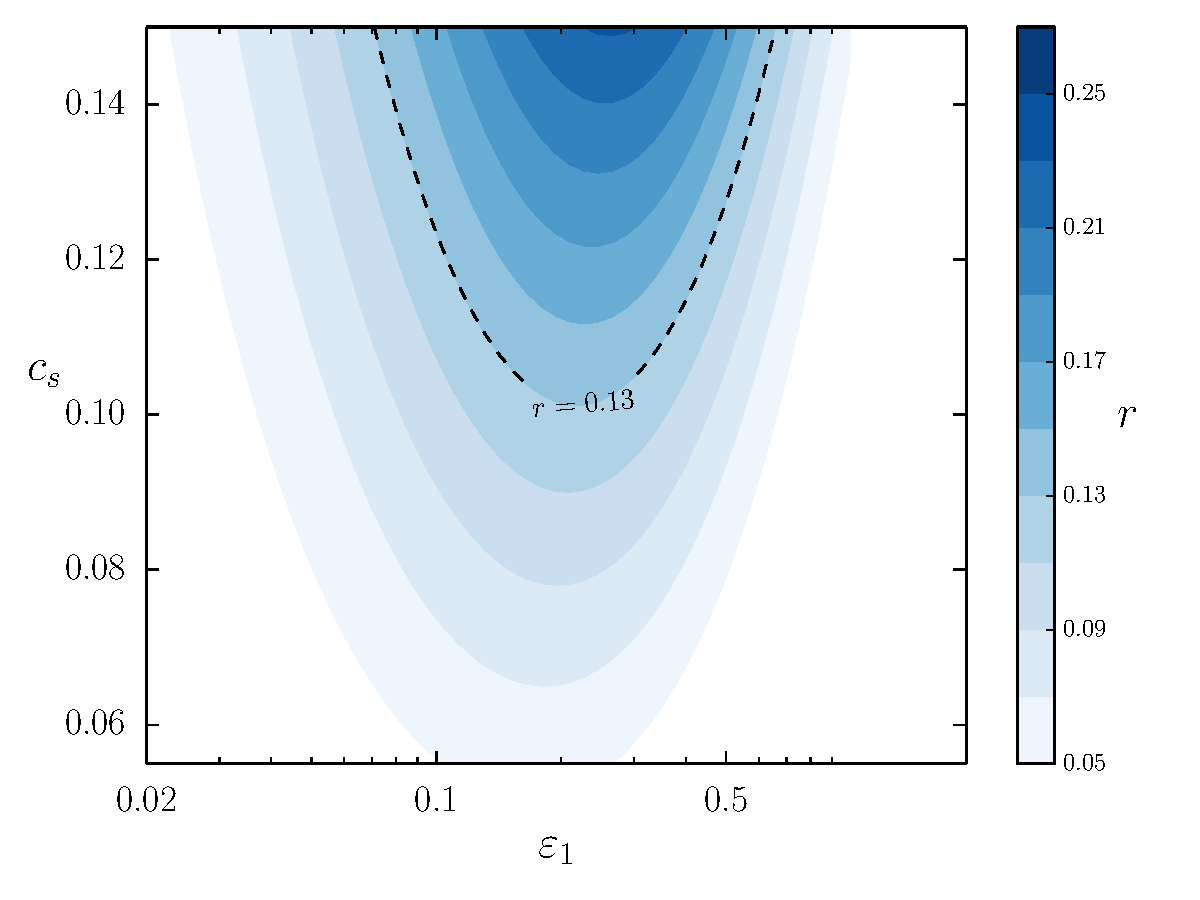
\includegraphics[width=0.65\textwidth]{rcs}
\caption{This is the figure we made last time. }
\label{figurename}
\end{center}
\end{figure}
The This is a reference to figure \ref{figurename}.

\subsection{Tables}

The last basic object is a table (which is basically like a matrix)

A basic examples with has everything is this.  It iw a big confusing because l, r and c refer to justification where | (pipe or the vertical line) is how we want vertical lines to appear between columns.  hline implements all the horizontal lines in your table. 

\begin{table}[h!]
\begin{center}
  \begin{tabular}{ | l || c ||| r  |}
    \hline
    1 & 2 & 3 \\ \hline
    4 & 5 & 6 \\ \hline \hline
    7 & 8 & 9 \\
    \hline
  \end{tabular}
\end{center}
\caption{This is a table}\label{tablename1}
\end{table}
One extra feature is that sometimes you what a horizontal that only goes from element i to j.  To do this we use cline 
\begin{table}[h!]
\begin{center}
  \begin{tabular}{ | l | c  r  |}
    \hline
    1 & 2 & 3 \\ \cline{2-3}
    4 & 5 & 6 \\ \hline 
      7 & 8 & 9 \\
    \hline
  \end{tabular}
  \
\end{center}
\caption{This is another table}\label{tablename2}
\end{table}

And of course, we can refer to table \ref{tablename1} and \ref{tablename2} as usual.
\section{Compiling latex with bibtex}

The second most annoying feature of latex is it takes 4 compiles to get it to look right.  To compile you need to run the four commands in your terminal:
\bea
&\text{latex template.tex}&\\
&\text{bibtex template}&\\
&\text{latex template.tex}&\\
&\text{latex template.tex}&
\eea
If you download texshop, you need to press typeset with Latex, then Bibtex, the Latex twice.

This is the price you pay for having proper management of your references.  Bibtex automatically includes only the references cited in the text and numbers them in the order they appear.  Doing this by hand is a giant point which is worth the 4 compiles to avoid.
\appendix
\section{An appendix}


\newpage
\addcontentsline{toc}{section}{References}
%\va{check bibliography, in particular capital letters in titles}
\bibliographystyle{utphys}
%\bibliographystyle{kp}
\bibliography{template}
\end{document}
